\section{Results and Discussion}

The initial phase of our project was dedicated to cleaning and validating the Anatomy Registers dataset. Given the large volume and arcane lettering of the handwritten records, the dataset was prone to numerous transcription errors. Our systematic approach, involving techniques such as regular expressions, was critical for enhancing the data's reliability and accuracy, making it suitable for further analysis. 

Following data validation, we focused on data transformation and feature extraction, particularly targeting the ``place of death'' attribute. This involved (a) categorising each entry by the type of institution the patient died in (e.g. private residence, public hospital etc.), and (b) extracting the suburb where the patient died in. This involved using text parsing and geographic information system (GIS) techniques, which facilitated the transition from basic descriptive statistics to a deeper geospatial analysis. The refinement of this data allowed us to generate comprehensive choropleth maps, illustrating the distribution and evolution of donor sources across NSW. 

The animated choropleth map (Figure \ref{fig:choropleth-comparison}), showing the most common category of death place per suburb through each decade from the 1880s to 1980s, revealed a notable shift in the sources of bodies for anatomical study. Prior to 1950, a majority of bodies originated from public and mental asylums, indicating a period when body donation was more stigmatised and the Medical School was heavily reliant on unclaimed bodies from such institutions for anatomical dissection. However, post-1960s, there was a significant increase in donors from private residences, indicating a shift in public perceptions towards body donation as a more accepted and personal choice. 

\begin{figure}[p]
    \centering
    \caption{A choropleth map showing the stark difference between the largely institution-reliant donor program in the 1950s and the influx of private donors in the 1960s.}
    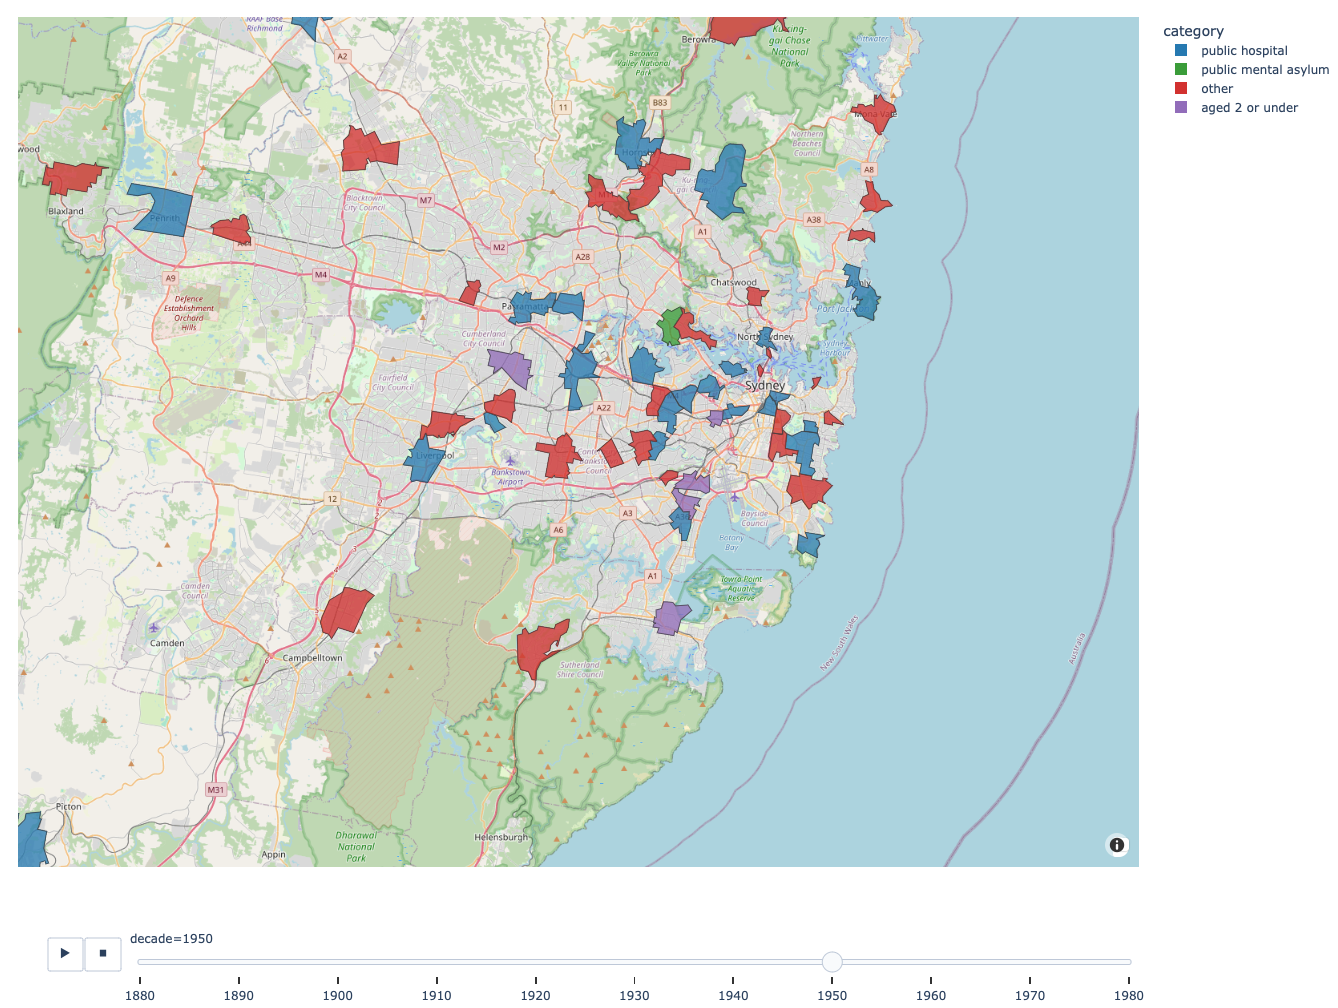
\includegraphics[width=0.95\textwidth]{REPORT/img/choropleth-1950.png}
    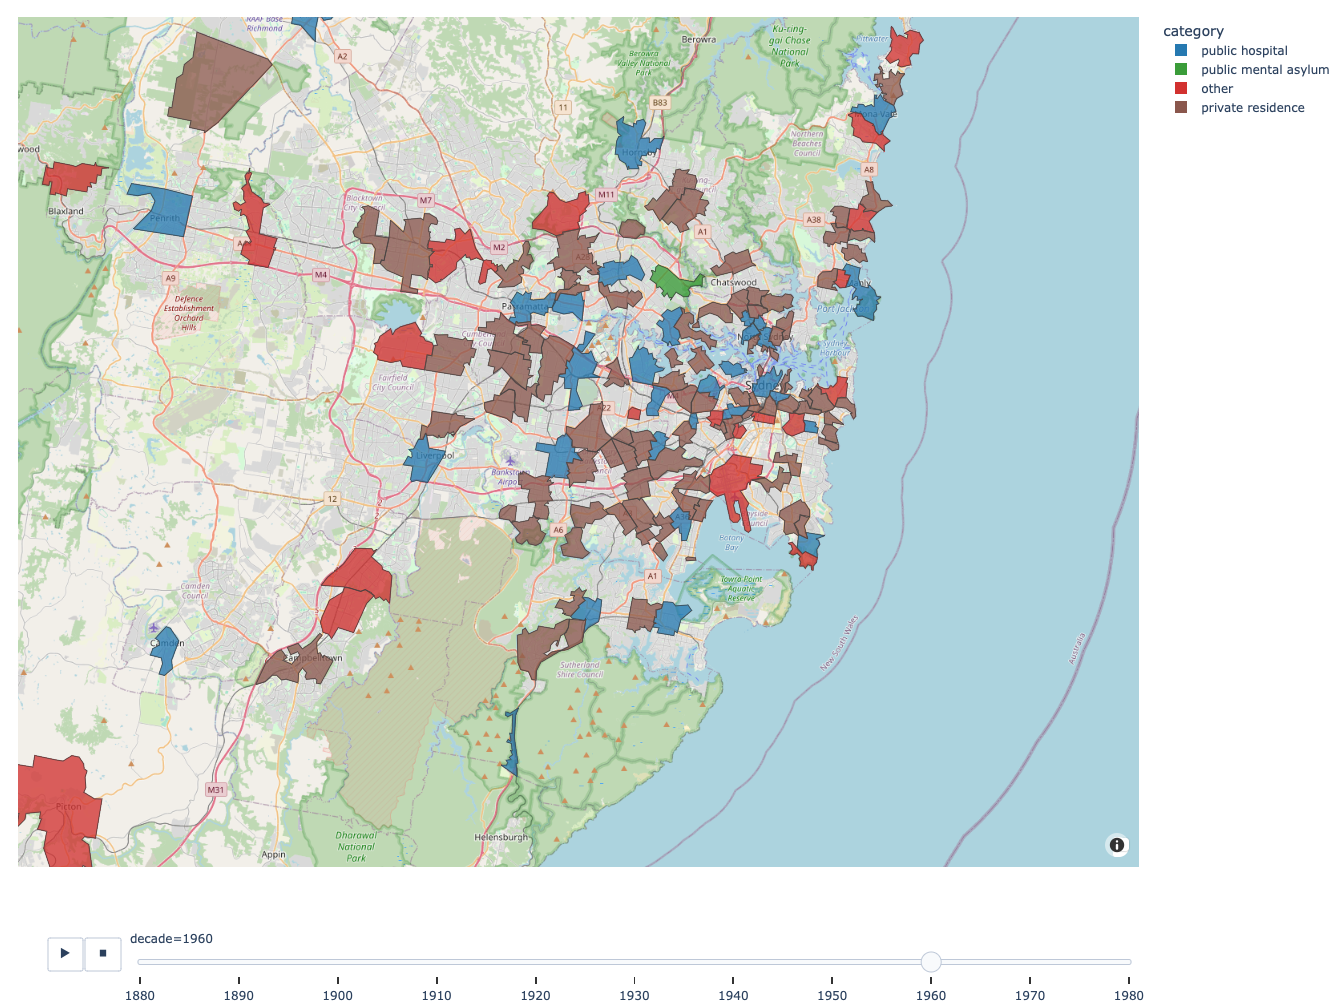
\includegraphics[width=0.95\textwidth]{REPORT/img/choropleth-1960.png}
    \label{fig:choropleth-comparison}
\end{figure}

This shift in attitude was coincident with the transition to a body donor program. Voluntary body donation steadily increased from the year 1916, when the first documented body donation was recorded, to the year 1960, where 118 out of 127 bodies admitted were registered or private donors, until ``by the late 1960s, a waiting list for would be donors had to be introduced, with restrictions on the registration of new donors sometimes lasting beyond a year'' \parencite{rebekah_jenkin}.

It appears that this trend of the public becoming more conscious over what happens to their body after they pass was not limited to just Australia. Indeed, Canada, the United Kingdom, and the United States also saw the upsurge of voluntary donation in the mid-20th century. In a similar study to the one conducted at the University of Sydney, anatomists at McGill University in Canada saw the first bequeathments (or ``gifts'' as they were originally called) of bodies in the 1950s and also witnessed the rate of donations increasing rapidly after the year 1965 \parencite{noel_2022_mcgill}. In the United Kingdom, it was in the late `40s that the newly-initiated National Health Service saw a ``dramatic'' change in public perceptions and saw the beginnings of bodies ``provided in a spirit of trust and generosity, by voluntary public donation'' \parencite{richardson_2006_ukdonors, jones_1991_nzdonors}. The United States also shared this trend despite limited ties to the UK and its legislature \parencite{garment_2007_usadonors}.\footnote{Canada and Australia's Anatomy Acts both aligned themselves closely to the original British Anatomy Act of 1832.} 

We cannot be certain for the reasons behind this uptrend in body donation during the 1950s and 1960s. This is because the way a society deals with death reflects the way its citizens live, and, as a result, any trends to due with bequeathment programs are a culmination of changes in society itself. 
\begin{quote}
A population boom, expansion of government, new legislation, changes in the population demographics, developments in science, and proliferation of mass media, all affected body acquisition. \parencite{garment_2007_usadonors}
\end{quote}
However, there are a few probable causes towards this trend.
\begin{enumerate}
    \item \textbf{The effects of World War II.} The widespread establishment of blood transfusion services during World War II had a profound influence on public willingness to contribute to medical science, not just through blood donation but also through body donation for dissection. As \citeauthor{richardson_2006_ukdonors} notes, the collective effort in wartime medical services likely fostered a sense of communal responsibility towards advancing medical knowledge and healthcare, which persisted into the post-war era \parencite{richardson_2006_ukdonors}. This shift contributed to a greater acceptance of body donation as another form of contribution to the medical field.
    \item \textbf{Shifts in religious beliefs.} The mid-20th century witnessed significant shifts in societal and religious attitudes towards the human body post-mortem. As traditional views on the spiritual significance of the corpse began to wane, alongside an increase in the popularity of cremation, public attitudes towards scientific medicine and body donation started to change. \citeauthor{jones_1991_nzdonors} touch on how these evolving beliefs, coupled with an enhanced understanding of the medical benefits of body donation, led to broader acceptance and support of anatomical donations \parencite{jones_1991_nzdonors}.
    \item \textbf{The cost of dying.} The American funeral industry boomed due to the popularisation of embalming in the mid-19th century, and alongside this, the price of funerals skyrocketed. According to \citeauthor{garment_2007_usadonors}, three pieces of journalism were instrumental in bringing to light the excessive costs paid to die in the country: ``The High Cost of Dying'' by Bill Davidson, ``Can You Afford to Die'' by Roul Tunley, and ``The American Way of Death'' by Jessica Mitford, all published in the `50s and `60s. Mitford's book contained the first publicly available list of schools that would accept bodies for donation, provided as an alternative to succumbing to exorbitant funeral costs. It is likely that Davidson, Tunley, and Mitford's works helped increase the public's awareness of alternatives, a key one being body donor programs.
\end{enumerate}


These insights into historical and societal trends are crucial as they highlight the impact of digitising and analysing historical datasets, echoing the broader themes discussed in our literature review. Just as the analysis of ship logbooks \parencite{petrakis_2021_ship} provided a window into the psychological landscape of historical maritime transitions, our project shows the evolution of societal attitudes towards a once-stigmatised aspect in medical science.

\subsection{Limitations}
Despite our achievements, the project faced certain limitations, particularly in the categorisation of the `place of death' entries. A significant number of entries remained classified under ``Other'', including those with misspelled addresses and ambiguous locations, indicating the complexity of interpreting such historical data accurately. This limitation underscores the need for more advanced natural language processing techniques and machine learning models to handle the intricacies of data entry. Additionally, manual review and enhancement of the categorisation process would likely improve data accuracy and the quality of insights derived from our analysis.